\documentclass[aspectratio=169]{beamer}
\usepackage[T1]{fontenc}
\usepackage[english]{babel}
\usepackage{booktabs}

\usetheme{Madrid}
\usecolortheme{beaver}
\setbeamertemplate{navigation symbols}{}

\title{{{TITLE}}}
\subtitle{Subtitle of the presentation}
\author{{{AUTHOR}}}
\institute{Institution}
\date{\today}

\begin{document}

\begin{frame}
  \titlepage
\end{frame}

\begin{frame}{Outline}
  \tableofcontents
\end{frame}

\section{Introduction}

\begin{frame}{A slide}
  Each slide is a \texttt{frame} environment.
  \begin{itemize}
    \item Lists are shown in full\ldots
    \item<2-> \ldots or one item at a time, with \texttt{<2->}.
  \end{itemize}
\end{frame}

\section{Content}

\begin{frame}{Two columns}
  \begin{columns}
    \column{0.5\textwidth}
    Text on the left, a figure or a table on the right.
    \begin{block}{Key point}
      Blocks bring an idea forward.
    \end{block}

    \column{0.45\textwidth}
    \centering
    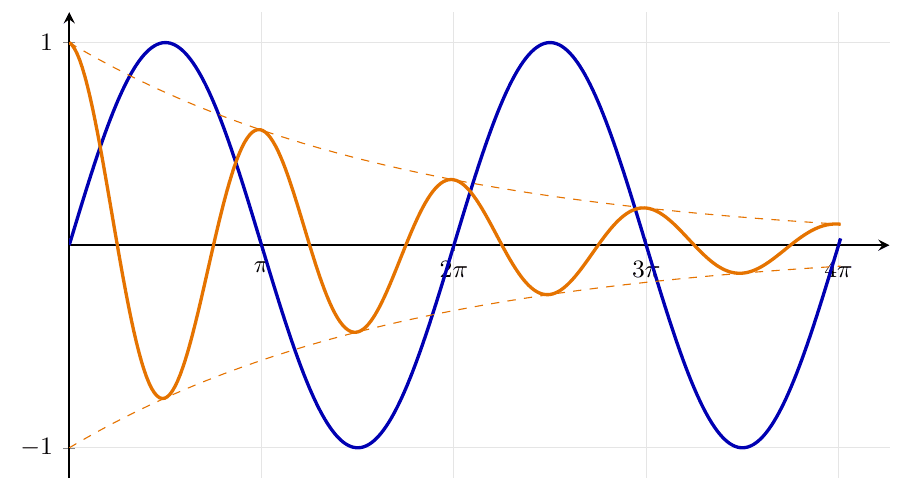
\includegraphics[width=\linewidth]{images/curves.png}
  \end{columns}
\end{frame}

\begin{frame}{Mathematics and a table}
  \begin{equation*}
    \hat{\beta} = (X^\top X)^{-1} X^\top y
  \end{equation*}
  \begin{center}
    \begin{tabular}{lrr}
      \toprule
      Method & Time (s) & Error (\%) \\
      \midrule
      A & 1.2 & 3.4 \\
      B & 0.8 & 2.9 \\
      \bottomrule
    \end{tabular}
  \end{center}
\end{frame}

\section{Conclusion}

\begin{frame}{Conclusion}
  \begin{alertblock}{Main message}
    The last slide recalls what matters most.
  \end{alertblock}
  \vfill
  \centering
  Thank you! Any questions?
\end{frame}

\end{document}
